\documentclass{beamer}

\usepackage{default}

\usepackage[english]{babel}
\usepackage[utf8x]{inputenc}

\title[Your Short Title]{Uncertainty Quantification: Prob, Drop, Det}
\author{You}
\institute{Where You're From}
\date{\today}

\begin{document}
	
	\begin{frame}
		\titlepage
	\end{frame}
	
	% Uncomment these lines for an automatically generated outline.
	%\begin{frame}{Outline}
	%  \tableofcontents
	%\end{frame}
	
	\section{Probabilistic approaches}
	\begin{frame}{\cite{gal_dropout_2015}'s test-time dropout}
		content...
	\end{frame}
	
	\begin{frame}{\cite{gast_lightweight_2018}'s \textit{ProbOut}}
		content...
	\end{frame}
	
	\section{The task under consideration}
	\begin{frame}{The inverse problem}
		content...
	\end{frame}
	
	\section{Architectures}
	\begin{frame}{Architecture overview}
		\begin{figure}
		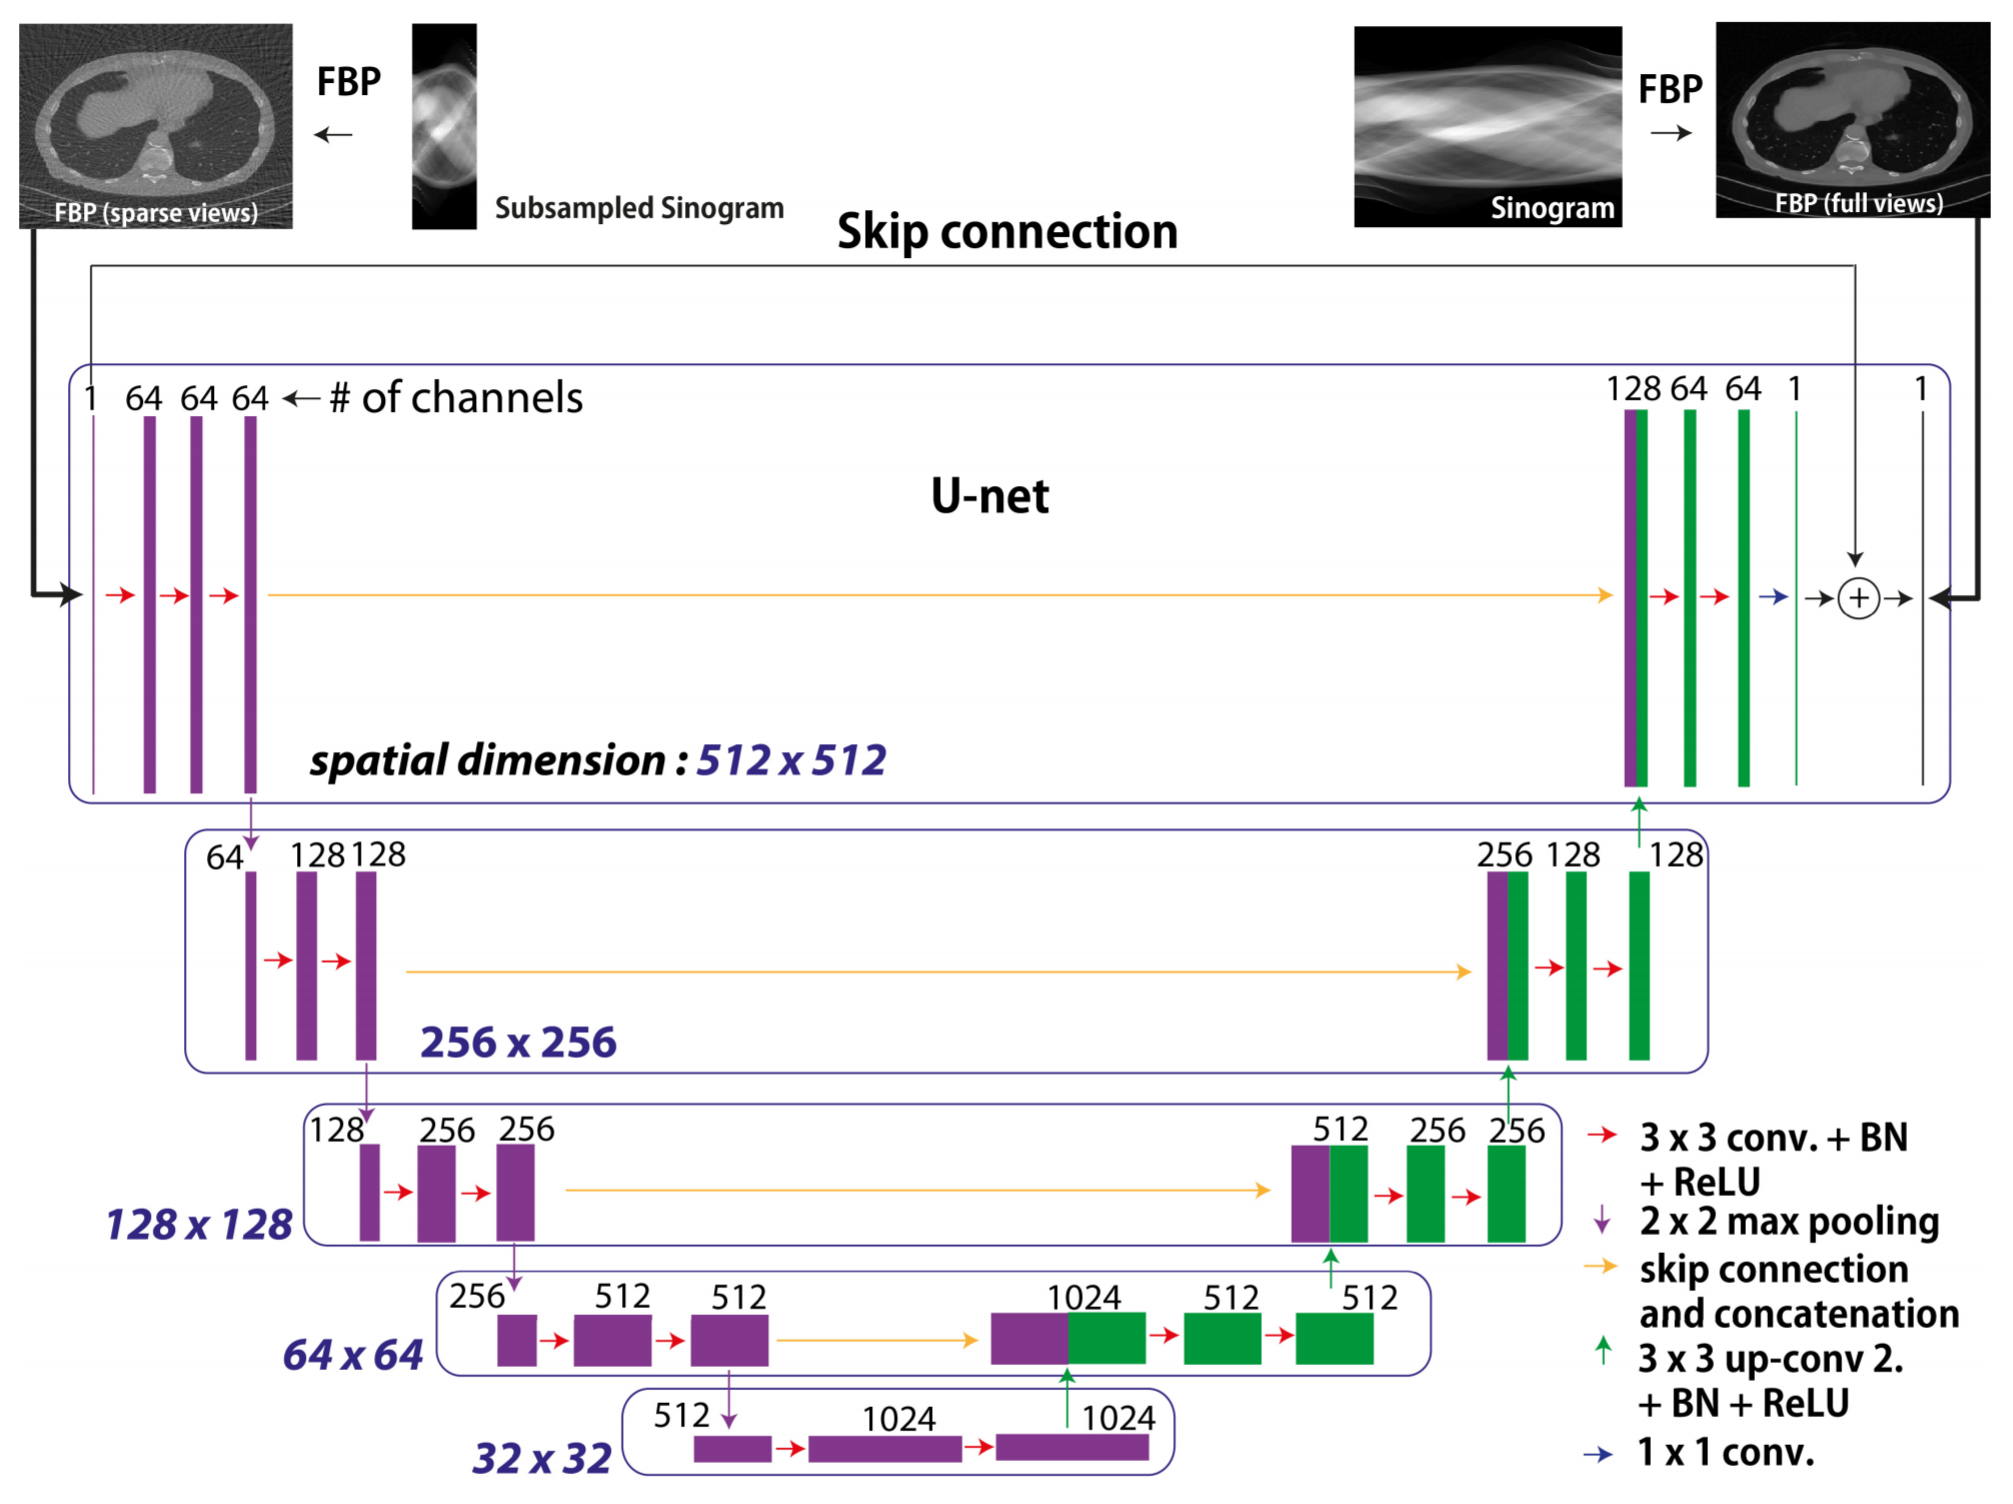
\includegraphics[width=0.8\textwidth]{figures/jin-unet.png}
		\caption{\label{fig:jin-unet}U-net as adapted by \cite{jin_deep_2017}, graph is by them.}
		\end{figure}
	\end{frame}
	
	\begin{frame}{Architecture variants}
		\begin{itemize}
			\item \textbf{FBPConvNet-Det}: the \cite{jin_deep_2017} et al model with l2 loss
			\item \textbf{FBPConvNet-Drop}: same as \textbf{FBPConvNet-Det}, but dropout is kept on during inference as proposed in \cite{gal_dropout_2015}
			\item \textbf{FBPConvNet-Prob}: at the last convolution one more kernel is added so that we get two outputs per datapoint, $\boldsymbol{\mu}$ and $\boldsymbol{\beta}$, and the l2 loss is replaced by the negative conditional log-likelihood of the power exponential distribution with $k=0.5$ $$-\log p(\mathbf{y}|\boldsymbol{\mu}, \boldsymbol{\beta}) \propto\sum_{d=1}^D \log \beta_d + (\sum_{d=1}^D \frac{(y_d - \mu_d)^2}{\beta_d})^k$$
			
		\end{itemize}
	\end{frame}
	
	
	
	\section{Bibliography}
	\begin{frame}[allowframebreaks]{Bibliography}
		\bibliographystyle{apalike}
		\bibliography{references/lib}
	\end{frame}

\end{document}
